\paragraph{}
%explicar separacion de partes entre oscilador y quench signal
El diseño del receptor se ha de separar en tres partes diferenciadas.
\paragraph{}
En primer lugar, la parte correspondiente al punto de operación de los transistores, tanto del oscilador de RF como del amplificador de la señal de \textit{quench}. En este apartado se trabaja con la componente DC.
\paragraph{}
En segundo lugar, se desarrolla la parte de RF correspondiente al oscilador, el cual define la frecuencia de trabajo. 
%\paragraph{}
%En tercer lugar, se desarrolla la parte correspondiente al regulador de tensi\'on de +\SI{5}{\volt}.
\paragraph{}
Por último, la parte correspondiente a la \textit{quench-signal}, encargada de gestionar el paro y arranque de la oscilación. Esta parte trabaja a una frecuencia intermedia que puede diferenciarse de la parte de RF y de la componente DC.

\paragraph{}
El esquema completo del receptor se expone en la figura \ref{fig:rx}.
\begin{figure}[h]
    \centering
    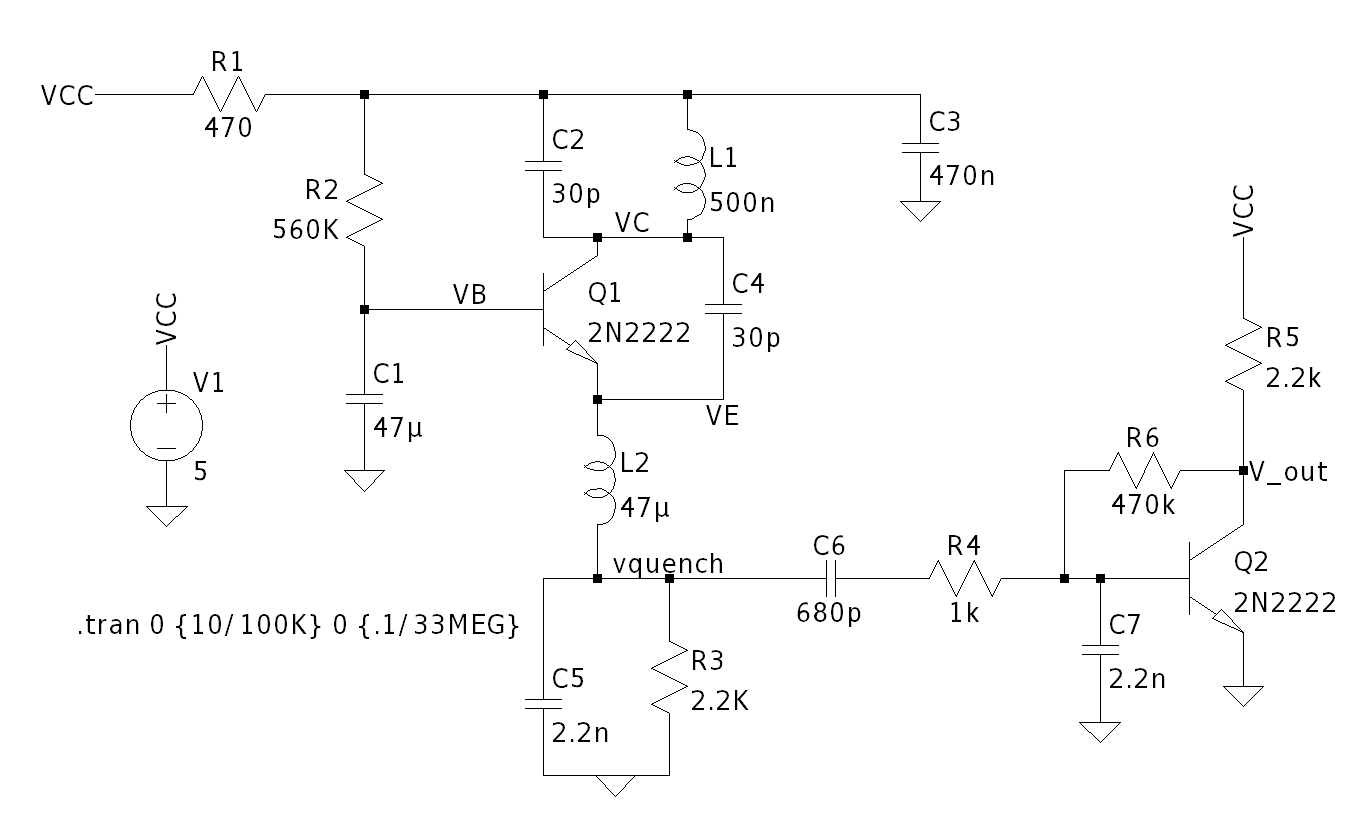
\includegraphics[scale=1, width=1\textwidth]{receptor}
    \caption{Esquema el\'ectrico del receptor}
    \label{fig:rx}
\end{figure}

\paragraph{Polarización} %EXPLICAR PORQUE ESE PUNTO DE OPERACION (MENOR RUIDO POSIBLE, MENOR CONSUMO DE POTENCIA)
\paragraph{}
En este caso, la estrategia para fijar el punto de operación es ligeramente distinta a como se diseña en el transmisor, pues se utiliza una estructura conocida como realimentaci\'on de colector. 
\paragraph{}
El transistor debe trabajar en zona activa directa, por lo que se debe cumplir $V_{CE} > V_{sat} \approx \SI{.2}{\volt}$ %se fijará $V_{CE} = \frac{V_{CC}}{2}$, para garantizar el mayor rango de linealidad posible.
Se fija tanto $V_{CC} = \SI{5}{\volt}$, como una corriente de colector aproximada de $I_C = \SI{600}{\micro\ampere}$, en este caso para que el transistor trabaje introduciendo el mínimo ruido posible.
Este hecho es importante, pues cuando el receptor se encuentra en la etapa de inicio de oscilación, un bajo nivel de ruido ayuda a aumentar la sensibilidad del receptor. Esto es debido a que la suma mínima de todos los ruidos generados por un transistor se encuentra en este rango de corriente de colector\footnote{Horowitz, P., \& Hill, W. (2015). \textit{The Art of Electronics} (Capítulo 8: Low Noise Techniques). Cambridge University Press.}.
Cabe recalcar, que la estructura de realimentación de colector provoca una realimentación negativa que fija el punto de operación de manera más independiente a los parámetros característicos del transistor. Esta realimentación negativa debe eliminarse en corriente alterna para provocar la oscilación. La estrategia para eliminarla se verá en el apartado de pequeña señal.
\paragraph{}
Se realizan los cálculos para estimar los valores de las resistencias de polarización en función de los valores anteriormente fijados. Las expresiones son v\'alidas para ambos transistores, pues poseen la misma configuraci\'on con diferentes valores.
\begin{align*} 
   I_i &= I_C + I_B = I_E \\
   I_i = I_E &= I_B \cdot (h_{FE} + 1) \\
   I_B \cdot (h_{FE} + 1) = I_E &= (h_{FE} + 1) \cdot \frac{V_{CE} - 0.7}{R_B} \\
   V_{CC} - V_{CE} - I_E \cdot R_E - I_E \cdot R_C &= 0 \\
   V_{CE} \cdot \left( 1 + \frac{(h_{FE} + 1) \cdot (R_E+R_C)}{R_B} \right) &= V_{CC} - \frac{0.7 \cdot (R_E+R_C) \cdot (h_{FE} + 1)}{R_B}
\end{align*}
\paragraph{}
De las anteriores expresiones se obtiene, para el transistor oscilador:
\begin{equation}
%   \label{eq:Al_tx}
   V_{CE} = \SI{1.74}{\volt} \quad \quad I_C = \SI{518}{\micro\ampere}
\end{equation}
\paragraph{}
Y para el transistor amplificador de la señal de \textit{quench}:
\begin{equation}
%   \label{eq:Al_tx}
   V_{CE} = \SI{1.76}{\volt} \quad \quad I_C = \SI{633}{\micro\ampere}
\end{equation}

\paragraph{Modelo en pequeña señal}
\paragraph{}
La estructura del oscilador en el receptor es idéntica al transmisor. 
En primer lugar, para evitar la realimentación negativa provocada por la parte de polarización, se coloca el condensador $C_3 = \SI{470}{\nano\farad}$. Este valor es suficiente para que su impedancia para la frecuencia de RF suponga un cortocircuito a tierra. La inclusión de este condensador es imprescindible para que el circuito funcione. 
\paragraph{} 
Debido a que el diseño es estructuralmente igual que en el transmisor, los cálculos serán idénticos sustituyendo los valores correspondientes.
Se incluyen los valores característicos junto a las ecuaciones de interés.
En función de los valores del punto de operación obtenido, se calculan los parámetros híbridos para el receptor.

\begin{equation}
   \label{eq:result_pol1}
V_{AF} = \frac{I_{Cdata}}{h_{OEdata}} =\frac{\SI{1}{\milli\ampere}}{\SI{6}{\micro\siemens}} =  \SI{50}{\volt} 
\end{equation}
\begin{equation}
   \label{eq:result_pol2}
%\[
\begin{array}{rl} 
      \begin{array}{l}
	 h_{ib} =  \SI{1.35}{\kilo\ohm} \\
	 h_{fb} =  -0.996
      \end{array}
      &
      \begin{array}{l}
	 h_{rb} =  0.014 \\
	 h_{ob} =  \SI{36.9}{\nano\siemens}
      \end{array}
\end{array}
%\]
\end{equation}

\paragraph{}
El modelo en pequeña señal para las frecuencias de RF es sustancialmente igual a la parte del transmisor (apartado \ref{des_tx.tex}). En la figura \ref{fig:ss_rx}, se muestra el modelo del receptor en pequeña señal para las frecuencias de RF. $L_2$ tiene una impedancia suficientemente grande como para considerarla circuito abierto. El objetivo del modelo es la obtención de una expresión para la frecuencia de resonancia.

\begin{figure}[h]
    \centering
    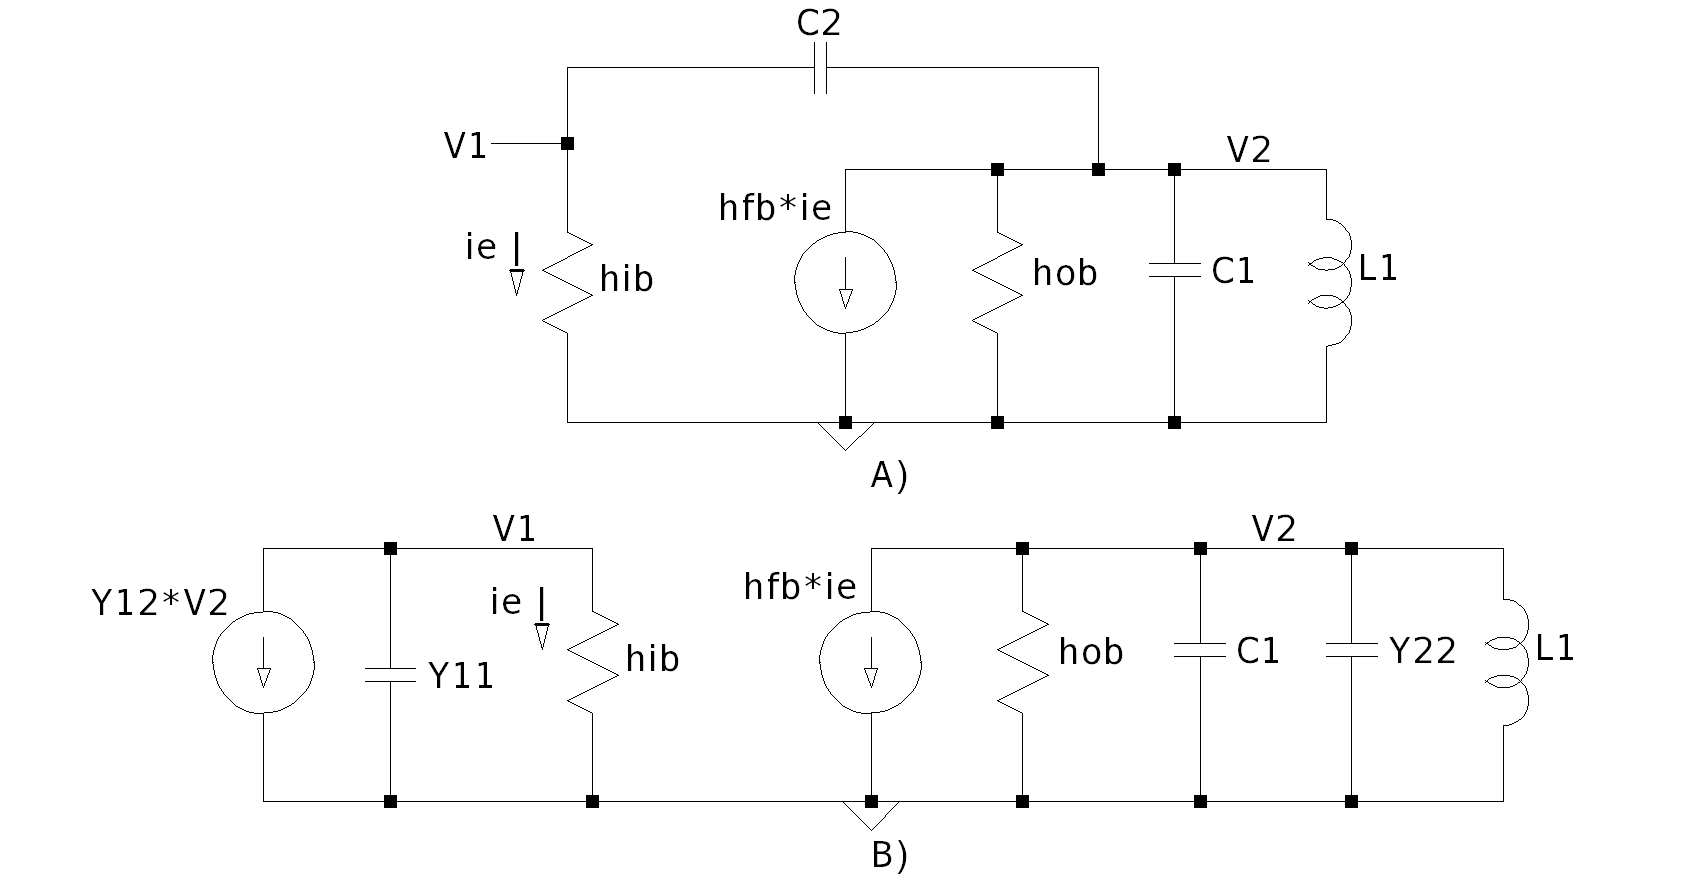
\includegraphics[scale=1, width=.8\textwidth]{small_signal_rx}
    \caption{A) Modelo en pequeña señal del bucle de oscilación para frecuencias de RF B) Modelo en pequeña señal del oscilador sustituyendo el condensador de realimentación $C_2$ por su equivalente en parámetros $Y$}
    \label{fig:ss_rx}
\end{figure}

%FALTA FUNCION DE TRANSFERENCIA IGUAL QUE TX Y CALCULO DE FREQ RESONANCIA IGUAL QUE TX. RAPIDAMENTE. DECIR QUE SE ANADE CONDENSADOR VARIABLE PARA SINTONIZAR ELUDIENDO LAS DISCREPANCIAS REALES DEL CIRCUITO.
\paragraph{}
Debido a la dualidad con respecto al tx, la expresión de la función de transferencia de lazo cerrado es idéntica al transmisor. La expresi\'on de la funci\'on de transferencia se muestra a continuaci\'on:

\begin{equation}
   \label{eq:Al_tx}
   A_l = \frac{h_{fb} \cdot C_1 \cdot s^2}{ \left( C_2+C_1 \right) \left( s \cdot h_{ib} \cdot C_2 + 1\right) \left( s^2 + s \cdot \frac{h_{ob}}{C_1 + C_2} + \frac{1}{(C_1 + C_2)\cdot L_1}\right) }
\end{equation}

\paragraph{}
Se obtiene la frecuencia de resonancia como: $$\omega_0^2 = \frac{1}{L_1 \cdot (C_1 + C_2)}$$
$$ f_0 = \frac{1}{2 \cdot \pi \cdot \sqrt{L_1 \cdot (C_1 + C_2)}} = \SI{30.63}{\mega\hertz} $$
\paragraph{}
El valor de la inductancia $L_1$ es el mismo que el calculado en el apartado \ref{sec:des_tx}, pues esta se construye con las mismas caracter\'isticas. El valor resultante es calculado mediante la ecuaci\'on \ref{eq:def_inductance2}:
$$ L_1 = \SI{450}{\nano\henry} $$


\paragraph{\textit{Quench-signal}} %AISLAR CIRCUITO, REALIZAR C\'ALCULOS, L(CHOKE) R Y C
\paragraph{}
En este caso, al contrario que en el receptor, la bobina de RFC no podrá ser arbitrariamente grande, pues debe permitir el paso de la frecuencia de \textit{quench} pero no de la señal de RF.
%El par RC provocan la oscilación de paro y marcha del circuito, pues al realizar los cálculos, se observa que sus valores fijan el coeficiente de amortiguación del sistema. 
%i think i have now understood, the value of L2 is critical because it needs to be as large as possible to be a high impedance for rf, but an intermediate impedance to quench. This quench frequency will be always the higher possible that could be amplified in the possitive loop and at the same time can pass in the low pass filter no?
\paragraph{}
En primer lugar, es necesario una explicación analítica del fenómeno para facilitar el entendimiento antes de realizar los cálculos de interés.
El transistor trabaja en configuración de base común. Esto implica que la tensión de base $V_B$ es fija, mientras que $V_E$ varía en el tiempo cortando y activando el transistor. Para un mejor entendimiento, se habla de $V_E$ como $V_{quench}$ indistintamente, pues $V_{quench}$ es $V_E$ tras el filtro paso bajo, eliminando visualmente la componente RF. La componente de baja frecuencia es quien corta el transistor de forma general. En la figura \ref{fig:quench-explain} se observa de forma gráfica la explicación dada a continuación.
\paragraph{}
Partiendo de una tensión $V_B - V_{quench} \approx \SI{0.7}{\volt}$, la oscilación comienza a generarse.
%Se toma como referencia $V_{quench}$ y no $V_E$ debido a que $V_E$ proporciona información tanto de las frecuencias de RF como las de frecuencia de quench, mientras que $V_{quench}$ proporciona la información de las frecuencias de interés por actuar como filtro paso bajo. 
%Mientras que la frecuencia de RF evidententemente satura y corta el transistor en numerosos ciclos por segundo, quien importa es quien corta la oscilación. 
A medida que la oscilación, al encontrarse dentro de un bucle de realimentación positiva, va incrementando su amplitud, la tensión media $V_{quench}$ también aumenta. En el momento que $V_{quench}$ aumenta de forma que $V_B - V_{quench} < \SI{0.7}{\volt}$, el transistor se corta, matando la oscilación y provocando que la tensión $V_{quench}$ descienda, volviendo de esta forma a completar el ciclo.
\paragraph{}
Para calcular la frecuencia de \textit{quench}, se debe tener en cuenta el filtro paso bajo formado por $L_2, C_5$ y $R_3$. 
Se calcula la función de transferencia del conjunto de estos tres elementos, al cual se le llamará cicuito de \textit{quench}.
Se pretende obtener la expresión para la función de transferencia de $H(s) = \frac{i_{L_2}}{v_i}$. 

\begin{align*} 
   v_i &= i_{L_2} \cdot ( Z_1 + Z_2 ) \\
   Z_1 &= s\cdot L_2 + r_s \\
   Z_2 &= \frac{R_3}{s \cdot R_3 \cdot C_5} \\
   \frac{i_{L_2}}{v_i} &= \frac{1}{( Z_1 + Z_2 )} = \frac{(s\cdot R_3 \cdot C_5 + 1)}{rs \cdot (s\cdot R_3 \cdot C_5 + 1) + s \cdot L_2 \cdot(s\cdot R_3 \cdot C_5 + 1) + R_3 } \\
\end{align*}

\begin{equation}
   \label{eq:Al_tx}
   H(s) = \frac{i_{L_2}}{v_i} = \frac{(s\cdot R_3 \cdot C_5 + 1)}{R_3 \cdot ( s\cdot r_s \cdot C_5 + s^2 \cdot L_2 \cdot C_5 + 1)}
\end{equation}
\paragraph{}
Se calcula la frecuencia de resonancia como $$\omega_0^2 = \frac{1}{L_2 \cdot C_5}$$
$$ f_0 = \frac{1}{2 \cdot \pi \cdot \sqrt{L_2 \cdot C_5}} = \SI{495}{\kilo\hertz} $$
%pero no en este caso la frecuencia de quench no se corresponde con la frecuencia de corte del filtro, ya que, el condensador no se descarga completamente en sus ciclos pues depende del transistor. 
\paragraph{}
En la figura \ref{fig:quench-explain}, se muestra por un lado, a la izquierda, la respuesta en frequencia del circuito de \textit{quench}, compuesto por: $L_2, R_3$ y $C_5$ en el esquemático del transmisor (figura \ref{fig:rx}). La respuesta en frecuencia es simulada para varios valores de $L_2$, y se indica con cursores. En el caso el caso de $L_2 = \SI{47}{\micro\henry}$, el valor de su frecuencia de corte es $f_c = \SI{483}{\kilo\hertz}$. 
\paragraph{}
Por otro lado, a la derecha, se muestra la simulación en función del tiempo del receptor. Se hace hincapié en la corriente de $L_2$. Esta está cursorizada de forma aproximada al valor que debería tener si a través de la bobina pudiera conducir corriente negativa, siendo este valor igual que el de la frecuencia de corte en la simulaci\'on en frecuencia.
La corriente de la inductancia $L_2$ no puede ser negativa, pues en este sentido de circulación la unión PN base emisor se encuentra inversamente polarizada y el condensador de realimentación tiene alta impedancia para frecuencias bajas. 

\begin{figure}[h!]
    \centering
    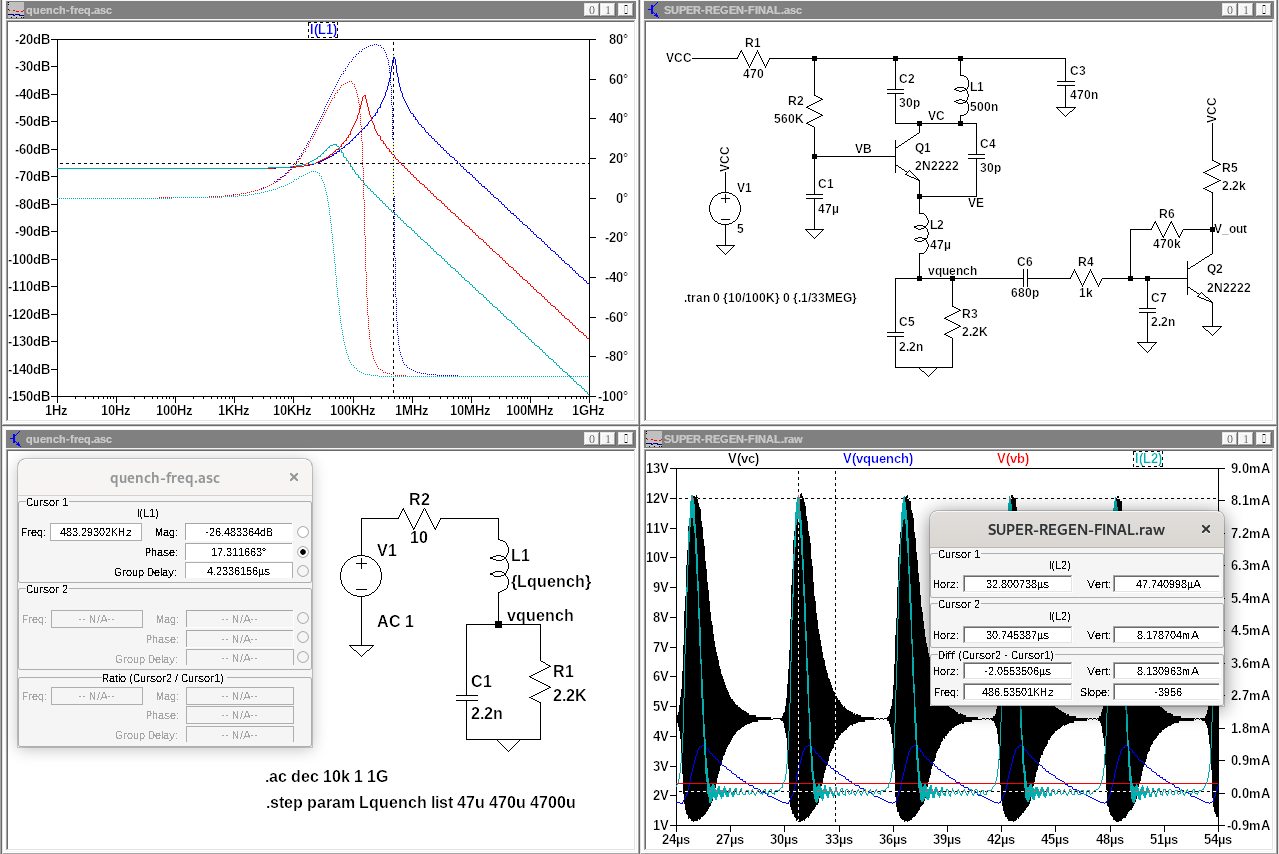
\includegraphics[scale=1, width=1\textwidth]{quench-explain}
    \caption{Explicación del comportamiento de la señal de quench}
    \label{fig:quench-explain}
\end{figure}

\paragraph{}
%REF Tipler pag 869. descarga condensador
En cualquier caso, la frecuencia real de \textit{quench} no es la calculada en la ecuacion \ref{eq:Al_tx}, sino que la señal de \textit{quench} se genera como se muestra en la figura \ref{fig:quench-explain}. 
En el momento que $i_{L_2} = 0$, la tensión en $V_{quench}$ se descarga a trav\'es de $R_3$, siguiendo $\tau$ de $C_3$ y $R_3$ hasta que $V_B - V_{quench} < 0.7$, reiniciando el ciclo.
El tiempo de subida depende tanto del tiempo que tarda en reconstruirse la oscilaci\'on como de la constante de elongación del sistema de la ecuación REF. Esta constante viene dada por $r_s$ y $C_5$ EXPRESION y define $v_{oi}$.
Se calcula aproximadamente la frecuencia de \textit{quench} siguiendo los valores de la figura \ref{fig:quench-explain}. 
\begin{align*} 
   i_{C_5} + i_{R_3} &= 0 \\
   C_5 \cdot \frac{dv_0(t)}{dt} + \frac{v_0(t)}{R_3} &= 0 \\
   \int_{v_{0i}}^{v_0(t)} \frac{1}{v_0(t)} \, dv_0(t) &= \int_{0}^{t} \frac{-1}{R_3 \cdot C_5} \, dt \\
\end{align*}

\begin{equation}
   \label{eq:des_rx-rc}
   ln \left( \frac{v_0(t)}{v_{oi}} \right) = \frac{-t}{R_3 \cdot C_5}
\end{equation}
\begin{equation}
%   \label{eq:Al_tx}
   \frac{v_0(t)}{v_{oi}} = e^{\left( \frac{-t}{R_3 \cdot C_5} \right)}
\end{equation}

\paragraph{}
Se usa \ref{eq:des_rx-rc} para calcular el tiempo de descarga con los valores de la figura \ref{fig:quench-explain}.
$$ t_{disch} = \SI{3.62}{\micro\second} $$
A este tiempo, se le debe sumar el tiempo de subida que viene dado por el tiempo de construcción de la oscilación junto con el tiempo de subida del sistema del circuito \textit{quench}.
Este tiempo, se aproximar\'a como $t_{rise} \approx t_{disch}$. Por lo que $$t_{quench} \approx 2 \cdot t_{disch}$$ y por tanto $$f_{quench} = \frac{1}{t_{quench}}  = \SI{138}{\kilo\hertz} $$
\paragraph{}
Empíricamente, esta frecuencia resulta en $f_{quench} = \SI{67}{\kilo\hertz}$. Esto es debido a que los valores en la simulación difieren bastante de la realidad, pero no las formas de onda. El ajuste de la frecuencia de \textit{quench} empírica se realiza probando distintos valores de $C_5$ y $L_2$, pues $R_3$ se fija al polarizar el transistor.

\paragraph{Resultado de la simulaci\'on} 
%Se muestran las medidas simuladas de tension de mayor inter\'es con la nomenclatura de la figura FIG RF
%captura de oscilacion de rf, v en rc y vout
%captura con senal de entrada vout cambia de frecuencia
\paragraph{}
En el apartado de simulación, se trata de obtener una representación gráfica de lo desarrollado anteriormente sobre el receptor. Por ello, en la figura REF se observan los puntos de interés del circuito como son $V_C$, $V_{quench}$ y $V_{B}$, además de añadir la diferencia$V_B - V_{quench}$ como $V(B,quench)$. Estas cuatro medidas son suficientes para entender el ciclo de paro y marcha del transistor.
\paragraph{}
Como se puede observar en la figura \ref{fig:simrx_zoom}, a medida que se construye la oscilación, el valor medio de la tensión de $V_{C}$ (es decir $V_{quench}$) aumenta hasta que, finalmente, la diferencia $V_B - V_{quench} < \SI{.7}{\volt}$ hace desaparecer la oscilaci\'on. Este corte provoca que el valor medio de $V_C$ descienda, y por tanto $V_{quench}$, provocando finalmente que la diferencia $V_B - V_{quench} > \SI{.7}{\volt}$, reactivando al transistor y reiniciando el ciclo de oscilaci\'on.

\begin{figure}[h!]
    \centering
    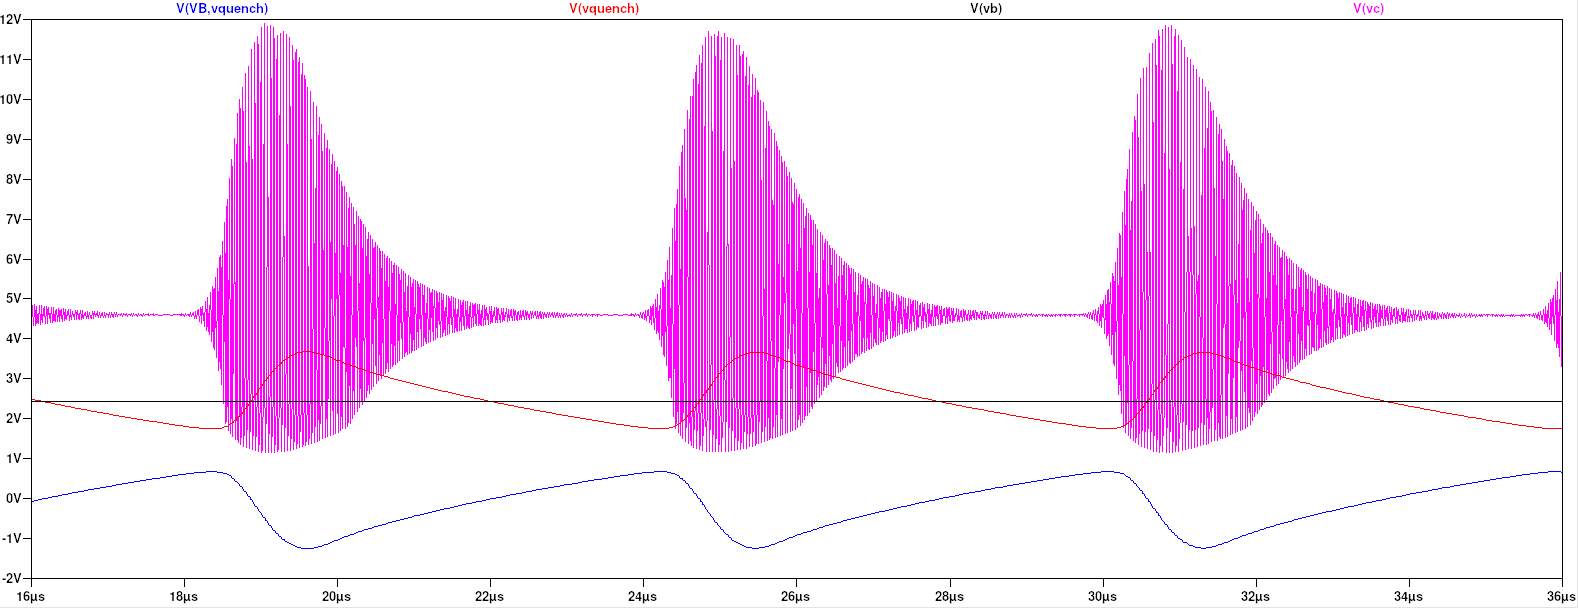
\includegraphics[scale=.8, width=.8\textwidth]{simrx_zoom}
    \caption{Simulación de los puntos de interés en varios ciclos ampliados}
    \label{fig:simrx_zoom}
\end{figure}

\paragraph{}
Se añade también, en la figura \ref{fig:simrx_vout}, la forma de onda de la tensión de salida $V_{out}$, que es la señal de entrada al microcontrolador atmega328p, el cual se encargará de demodular la señal. Esta señal debe ser una señal digital entre \SI{0}{\volt} y \SI{5}{\volt}.
\begin{figure}[h!]
    \centering
    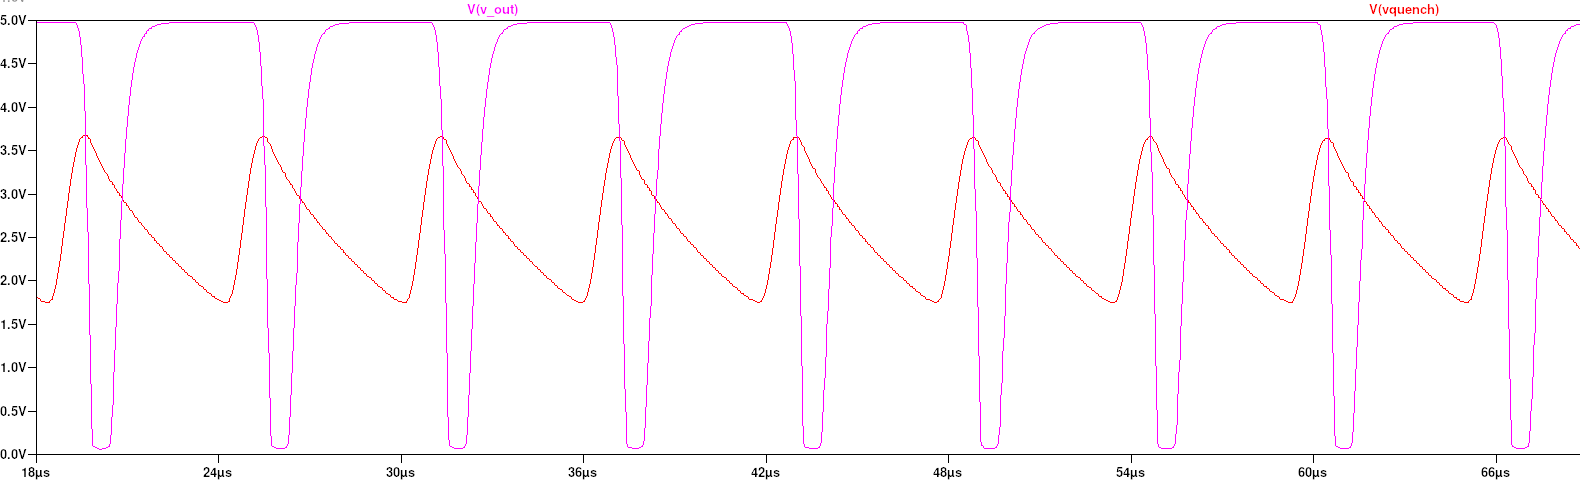
\includegraphics[scale=.8, width=.8\textwidth]{simrx_vout}
    \caption{Simulación de $V_{out}$ junto a $V_{quench}$}
    \label{fig:simrx_vout}
\end{figure}

\paragraph{Resultado práctico} 
\paragraph{}
En este caso se muestran las medidas tomadas en el apartado de simulaci\'on, esta vez tomadas en el circuito real. Las medidas se toman usando un osciloscopio digital. 
La configuración es la misma que en el en el apartado \ref{sec:des_tx} del transmisor. En este caso, al disponer de dos canales, se muestran en la figura \ref{fig:exp_vc_vquench} los puntos $V_{quench}$ (rojo) y $V_{C}$ (negro) y en la figura \ref{fig:exp_vout_vquench} los puntos $V_{out}$ (negro) y $V_{quench}$ (rojo).

\begin{figure}[h!]
    \centering
    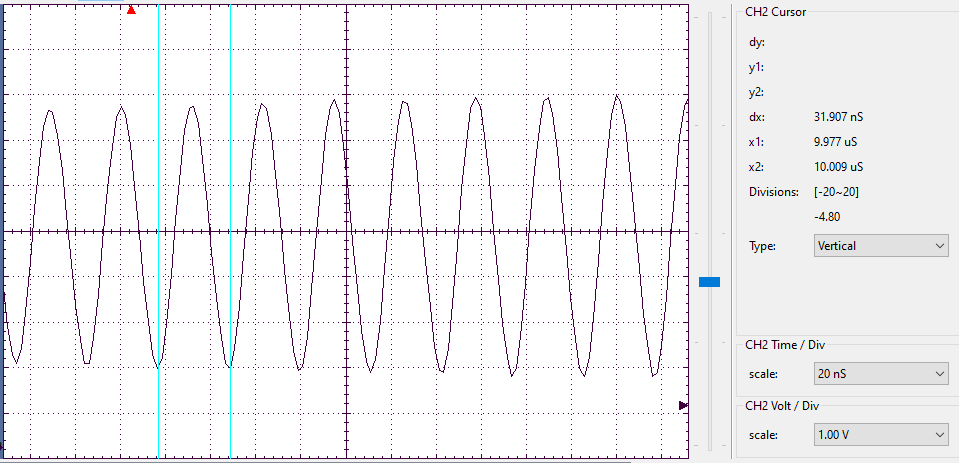
\includegraphics[scale=.7, width=.7\textwidth]{exp_work_freq.png}
    \caption{Experimental: captura de osciloscopio de la frecuencia de trabajo}
    \label{fig:work_freq}
\end{figure}
\begin{figure}[h!]
    \centering
    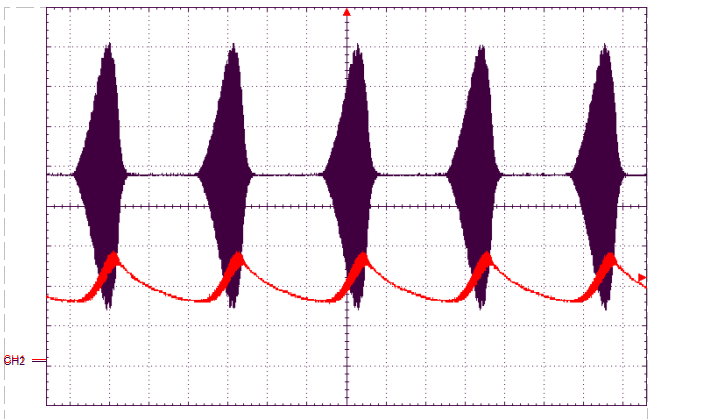
\includegraphics[scale=.7, width=.7\textwidth]{exp_quench+VC.PNG}
    \caption{Experimental: captura de osciloscopio de $V_C$ (negro) y $V_{quench}$ (rojo)}
    \label{fig:exp_vc_vquench}
\end{figure}
\begin{figure}[h!]
    \centering
    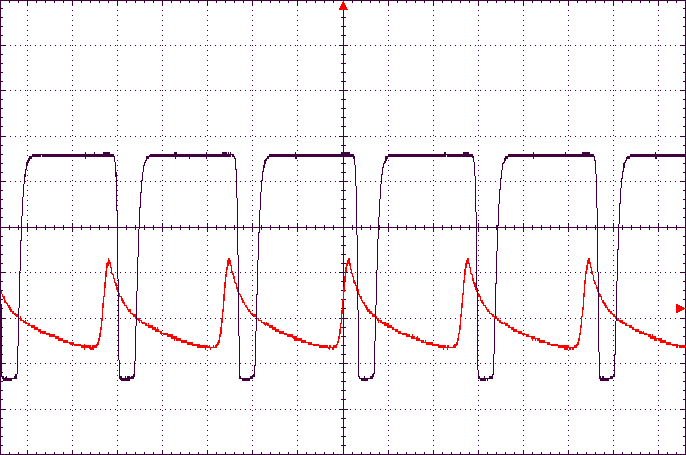
\includegraphics[scale=.5, width=.5\textwidth]{exp_quench+vout.png}
    \caption{Experimental: captura de osciloscopio de $V_{out}$ (negro) y $V_{quench}$ (rojo)}
    \label{fig:exp_vout_vquench}
\end{figure}

% situacion en el circuito (imagen bloque) y partes, enumeracion partes
% explicacion recepcion directa amplificando senal de RF y demodulando con filtro, posteriormente etapa de smith triger que se 
% manda al microcontrolador y detecta el canal. 
% \subsubsection{sintonizaci\'on y etapa de par Darlington}
% El circuito sintonizado que consigue la sensibilidad necesaria para captar la señal modulada proviniente del transmisor se consigue mediante un filtro paso banda sintonizado a la frecuencia de portadora. La corriente en la bobina $L_1$ producida por el campo electromagnético recibido, se amplifica notablemente a trav\'es de la etapa darlington, la cual, se encuentra polarizada con un $V_{CE}$ suficientemente bajo como para provocar la saturaci\'on del transistor ante la m\'inima intensidad de corriente en su entrada.
% \paragraph{Polarizaci\'on:} el par darlington debe ser lo suficientemente sensible como para poder detectar la corriente inducida en la bobina de recepci\'on, por lo que $I_B \approx \SI{28}{\nano\ampere}$
% \paragraph{Modelo en pequeña señal:} El objetivo de este apartado es el cálculo de la ganancia de la corriente de entrada con respecto a la tensión de salida de la etapa, y su impedancia de salida
% \subsubsection{Etapa en colector com\'un}
% Esta etapa actúa como un adaptador de impedancias de tal forma que la tensión de salida de la etapa darlington ataque a una impedancia de entrada alta para evitar pérdidas, mientras que la impedancia de salida de la etapa en colector común es baja y de ganancia en tensión similar a la unidad. A esta configuración se la conoce como \textit{"voltage buffer"}.
% \paragraph{Polarizaci\'on:} Se debe fijar una corriente de base del orden de la corriente que pueda proporcionar la etapa anterior, unos \SI{30}{\micro\ampere}. De forma an\'aloga a los anteriores apartados, se calcula el punto de operaci\'on para los valores del esquem\'atico, figura \ref{}
% \subsubsection{Amplificador de tensi\'on y filtro paso bajo}
% \subsubsection{comparador Smith triger}
% \subsubsection{Demodulaci\'on digital}
% demodulaci\'on digital a tr\'aves del microcontrolador se expondra en la sección 

